\begin{figure}[!htbp]
\caption{Legislator Ideal Points and District Ideology (Two Groups)}
\begin{centering}
%\centering
%\fbox{
  \begin{tabular}{@{}cc@{}}
	 & \\  
	\small (A) Marginal Effect of Percent Same-Party&	
  	\small (B) Marginal Effect of Same-Party Ideology\\
    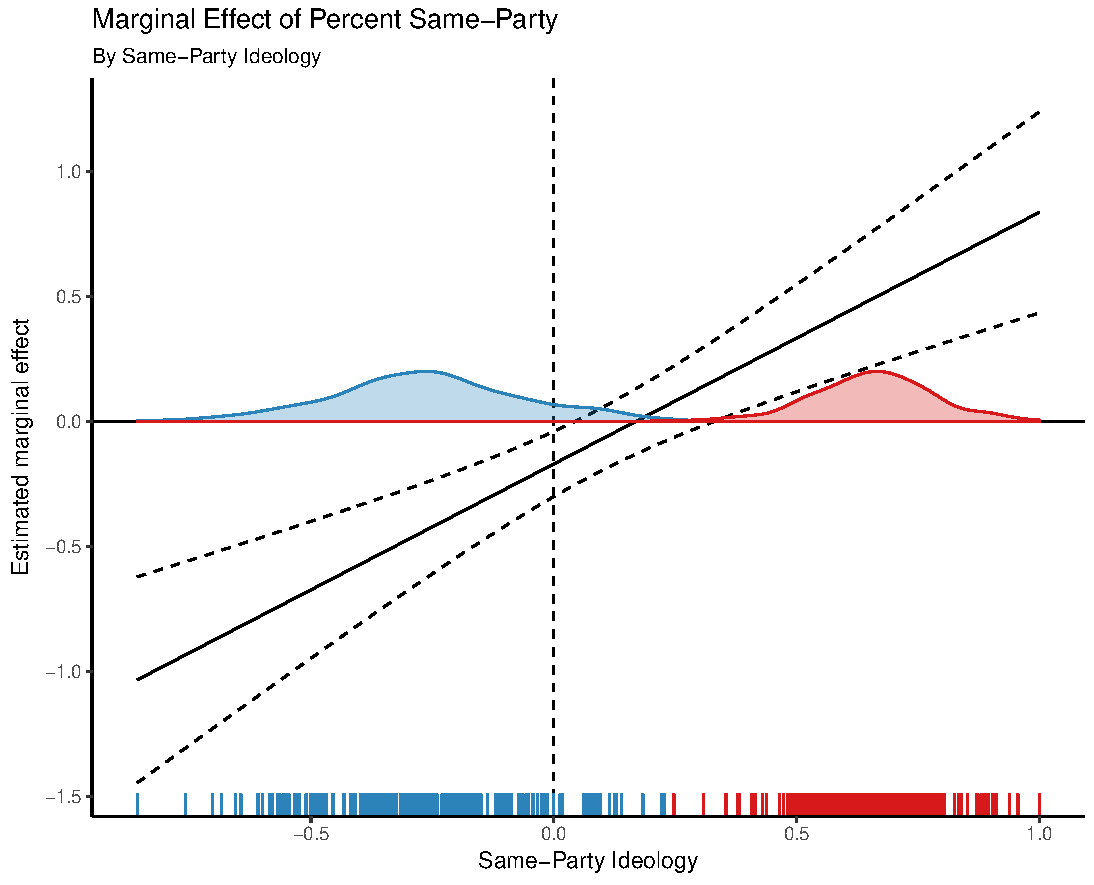
\includegraphics[width=.45\textwidth]{/Users/dsimp/GitHub/Clinton(2006)Rep/drafts/marginals/me-2.pdf} &
    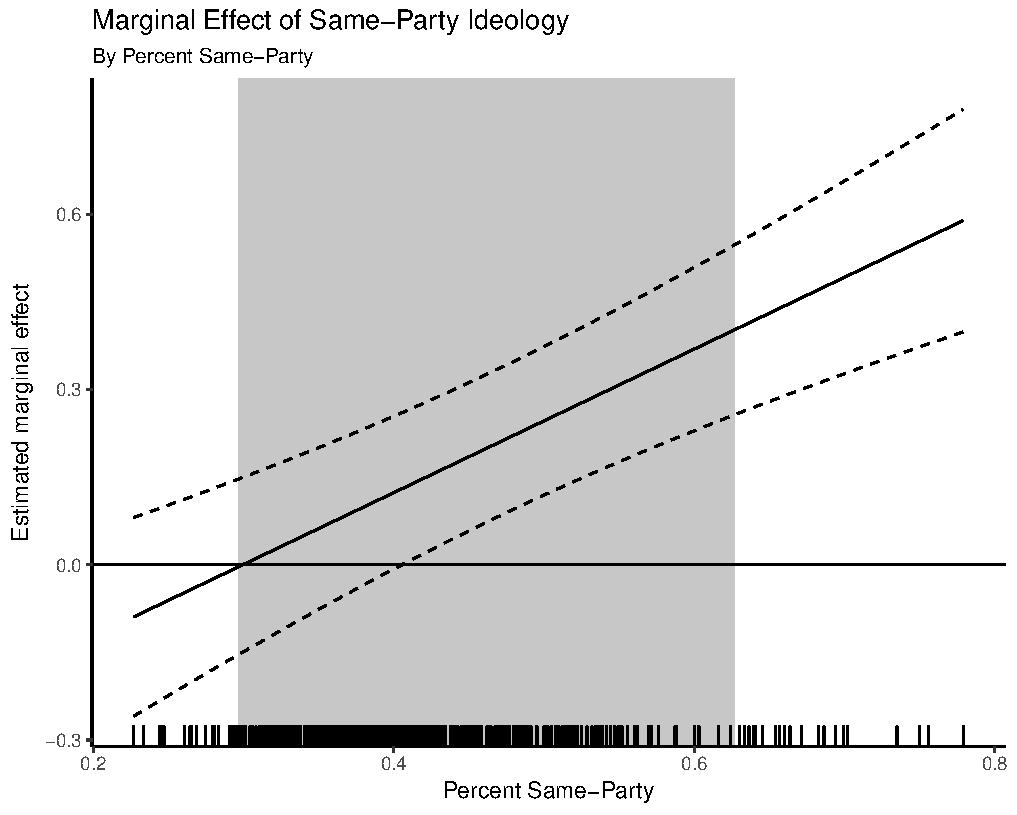
\includegraphics[width=.45\textwidth]{/Users/dsimp/GitHub/Clinton(2006)Rep/drafts/marginals/me-1.pdf} \\
     & \\
	\small (C) Marginal Effect of Percent Non-Same-Party& 
    \small (D) Marginal Effect of Non-Same-Party Ideology\\
    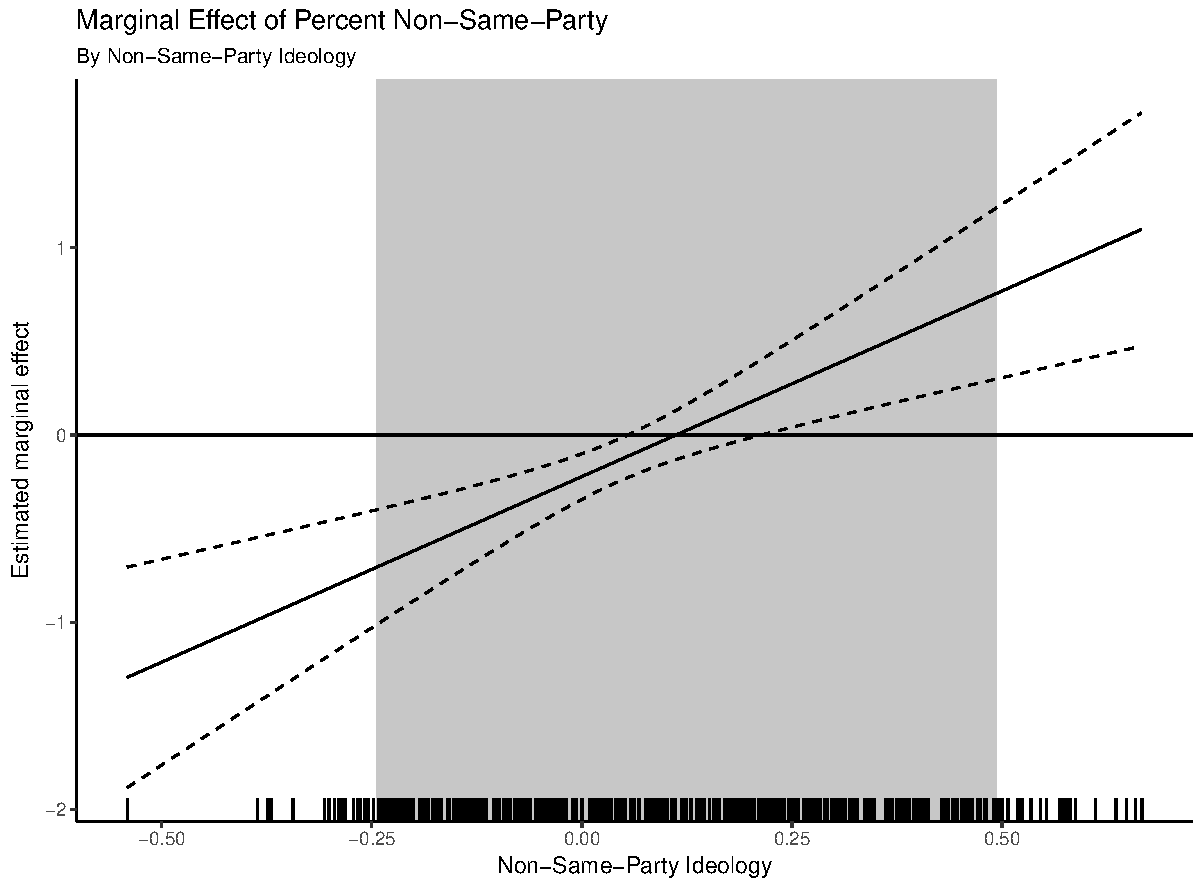
\includegraphics[width=.45\textwidth]{/Users/dsimp/GitHub/Clinton(2006)Rep/drafts/marginals/me-4.pdf} &
    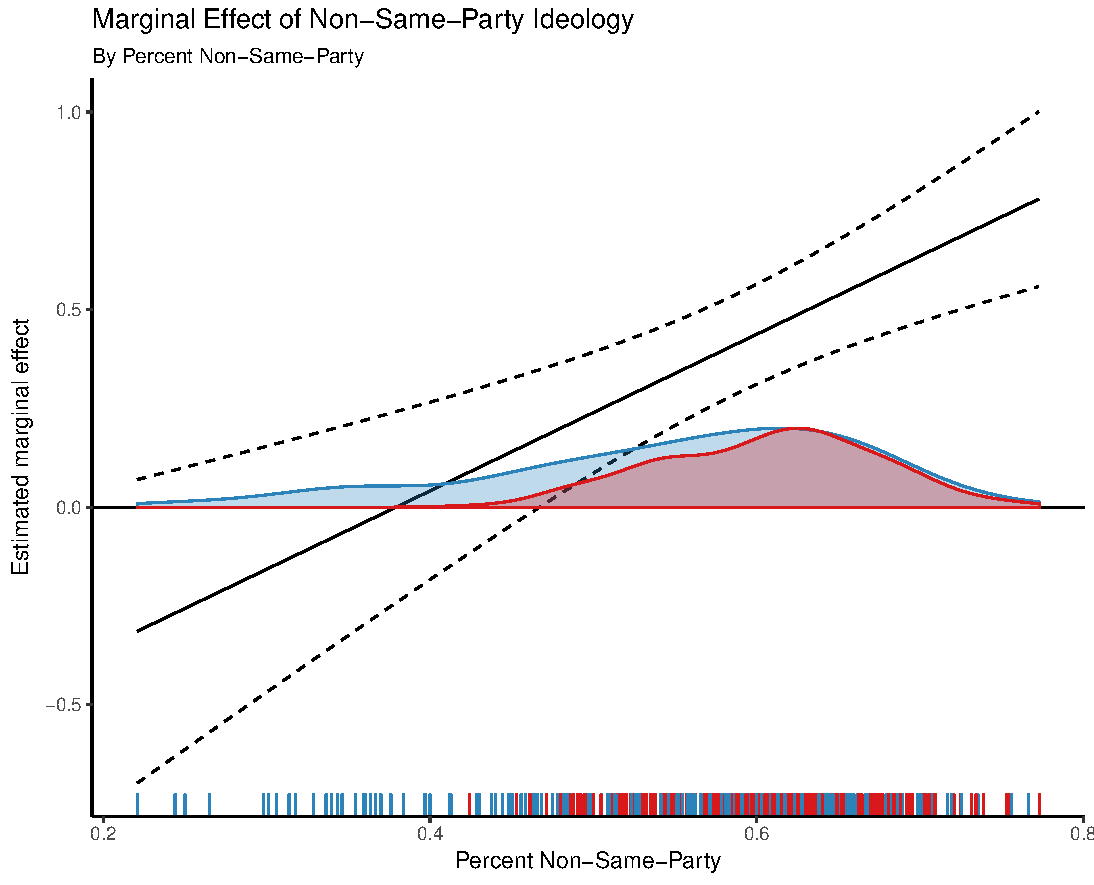
\includegraphics[width=.45\textwidth]{/Users/dsimp/GitHub/Clinton(2006)Rep/drafts/marginals/me-3.pdf} \\
     &  \\
  \end{tabular}
    %}   
 \end{centering}
  \textbf{Note:} Each panel plots the respective marginal effect of the constitutive terms of the interaction variables in Table 2 Model 3. The red (blue) distributions and rugs represent Republican (Democratic) held districts. \textbf{In future draft I will add a table with interval values to aid plot interpretation.}
\end{figure}
